\chapter{Вычислительные методы для теории представлений аффинных алгебр Ли}
\label{cha:computational-methods}

В данной главе мы описываем вычислительный пакет  {\bf Affine.m}, разработанный нами на основе идей и методов, изложенных в главах \ref{cha:affine-lie-algebras}, \ref{cha:BGG}. Этот пакет для популярной системы компьютерной алгебры {\it Mathematica} может использоваться для вычислений в теории представлений конечномерных и аффинных алгебр Ли. Реализованные в пакете алгоритмы основываются на свойствах весов и симметрии Вейля. Основные проблемы, которые может решать данный пакет -- это вычисление кратностей весов в неприводимых модулях и модулях Верма, построение правил ветвления и функций ветвления, а также разложение тензорных произведений. Такие задачи важны с точки зрения физических приложений (см. главы \ref{cha:CFT},\ref{sec:SLE}) и в данной главе мы приводим дополнительные примеры. 

Вычислительные методы в теории представлений имеют долгую историю \cite{belinfante1989survey}, существует большое количество программ и пакетов для вычислений, связанных с алгебрами Ли \cite{simplie}, \cite{vanleeuwen1994lsp}, \cite{stembridge1995mps,coxweyl}, \cite{fischbacher2002ilp}, \cite{Fuchs:1996dd}.

Большинство популярных программ \cite{simplie}, \cite{vanleeuwen1994lsp}, \cite{fischbacher2002ilp}, \cite{coxweyl} создано для изучения теории представлений простых конечномерных алгебр Ли. Здесь основные вычислительные задачи это:
\begin{enumerate}
\item Построение корневой системы, определяющей свойства алгебры Ли, в том числе коммутационные соотношения.
\item Перечисление элементов группы Вейля, необходимое ввиду симметрии корневой системы и характеров представлений относительно группы Вейля.
\item Вычисление кратностей весов, коэффициентов ветвления и слияния
\end{enumerate}
Существуют различные алгоритмы для решения этих задач \cite{moody1982fast}, \cite{stembridge2001computational}, \cite{belinfante1989survey}, \cite{casselman1994machine}.
Третья задача наиболее сложна с точки зрения вычислений. Существует два рекуррентных алгоритма, основывающихся на формуле Вейля для характеров и формуле Фрейденталя для кратностей. В данной главе мы их опишем.

Бесконечномерные алгебры Ли гораздо сложнее исследовать и число имеющихся программ гораздо меньше. 
Однако структура аффинных алгебр Ли позволяет адаптировать к ним вычислительные алгоритмы, предложенные для конечномерных алгебр Ли \cite{Fuchs:1996dd}, \cite{gannon2001algorithms}, \cite{kass1990ala}. В книге \cite{kass1990ala}, изданной в 1990 году, приведены таблицы кратностей весов неприводимых представлений и другие вычисленные характеристики аффинных алгебр и их модулей. Однако нам на данный момент не известны пакеты для популярных систем компьютерной алгебры, которые можно было бы использовать для воспроизведения и расширения этих результатов.

Чтобы исправить этот недостаток, нами был создан пакет {\bf Affine.m} для популярной системы  {\it Mathematica}. Возможности и ограничения этого пакета мы и описываем в этой главе. Кроме того, мы приводим некоторые примеры, связанные с физическими приложениями. 

Необходимые сведения из теории представлений приведены в главе \ref{cha:affine-lie-algebras}. Здесь мы начинаем с описания структур данных пакета  {\bf Affine.m}, использующихся для описания различных объектов теории представлений  (раздел \ref{sec:core-datastructures}), обсуждаем алгоритмы  (раздел \ref{sec:comp-algor}) и приводим примеры  (раздел \ref{sec:examples}). 

\section{Структуры данных}
\label{sec:core-datastructures} 
Хотя {\it Mathematica} -- нетипизированный язык программирования, в нем можно создавать структурированные объекты и проверять их типы используя сопоставление с шаблоном (pattern matching) \cite{shifrinmathematica}, \cite{maeder2000computer}.
\subsection{Веса}
\label{sec:weights}

Веса представляются двумя структурами данных: \lstinline{finiteWeight} для конечномерных алгебр Ли и \lstinline{affineWeight} для аффинных алгебр Ли.

Внутренняя структура веса конечномерной алгебры Ли представляет собой  \lstinline{List} с заголовком \lstinline{finiteWeight}, его компоненты -- это координаты веса в ортогональном базисе выбранном согласно Бурбаки \cite{bourbaki2002lie}.
Аффинный вес представляет собой расширение конечномерного веса с добавлением уровня и грейда. 

В пакете {\bf Affine.m} содержится набор функций для работы с весами конечномерных и аффинных алгебр Ли. Полный список доступен во встроенной справке пакета. Важнейшие из них -- это определение операций сложения, умножения на число и скалярного произведения (билинейной формы) для весов. В результате можно использовать традиционные обозначения при работе с  {\bf Affine.m}:
\begin{lstlisting}
  w=makeFiniteWeight[{1,0,3}];
  v=makeFiniteWeight[{3,2,1}];
  2*w+v==makeFiniteWeight[{5,2,7}]
  w.v==6
\end{lstlisting}

Использование ортогонального базиса во внутренней структуре весов позволяет нам работать с весами без полного задания корневой системы. Это полезно при изучении редукции на подалгебры, так как корни подалгебры можно задать вручную, путем указания их координат в ортогональном базисе.

\subsection{Корневые системы}
\label{sec:root-systems}

Чтобы задать конечномерную или аффинную алгебру достаточно определить ее корневую систему. Корневые системы представляются двумя структурами данных \lstinline{finiteRootSystem} и \lstinline{affineRootSystem}. Вторая структура является расширением первой. Мы предлагаем несколько конструкторов для этих структур данных. Во-первых, можно определить простое корни явно, например, при изучении вложения $B_2\subset B_4$ можно использовать определение
\begin{lstlisting}
  b2b4=makeFiniteRootSystem[ { {1,-1,0,0}, {0,1,0,0} } ]
\end{lstlisting}
Для корневых систем простых конечномерных алгебр Ли есть специальные конструкторы:
\begin{lstlisting}
  b2=makeSimpleRootSystem[B,2]
\end{lstlisting}
В графическом интерфейсе {\it Mathematica} можно использовать традиционные математические обозначения для простых алгебр Ли:


\begin{lstlisting}[mathescape=true]
  $B_2$ == makeFiniteRootSystem[ { {1, -1}, {0, 1} }]
\end{lstlisting}

Нескрученные аффинные корневые системы могут быть созданы как аффинные расширения корневых систем конечномерных алгебр Ли, например:
\begin{lstlisting}
  b2affine = makeAffineExtension[b2]
\end{lstlisting}
В графическом интерфейсе это же определение можно ввести просто как $\hat{B}_2$.

Полупростые алгебры Ли представляют собой прямые суммы простых:
\begin{lstlisting}[mathescape=true]
  $A_1\oplus A_1$ == finiteRootSystem[2, 2, {finiteWeight[2, {1, 0}], finiteWeight[2, {0, 1}]}]
\end{lstlisting}
%% The problem is here

Предикат \lstinline{rootSystemQ} проверяет, является ли объект корневой системой конечномерной или аффинной алгебры Ли.

Список простых корней -- это определяющее свойство корневой системы, поэтому он доступен как \lstinline{rs[simpleRoots]}.

В пакете реализовано несколько функций для основных характеристик корневой системы. Вектор Вейля дается функцией
\lstinline{rho[rs_?rootSystemQ]}:
\begin{lstlisting}[label=list:1]
  In[1]  =  rho[b2]
  Out[1]  =  finiteWeight[2, {3/2, 1/2}]
\end{lstlisting}
Положительные корни строятся функцией  \lstinline{positiveRoots[rs_?rootSystemQ]}. Для аффинной алгебры Ли эта и аналогичные функции возвращают список до некоторого фиксированного грейда. Это максимальное значение грейда задается как свойство \lstinline{rs[gradeLimit]} и по умолчанию равняется 10. Список корней  (вплоть до грейда \lstinline{gradeLimit}) строится функцией \lstinline{roots[rs]}. Матрица Картана и фундаментальные веса вычисляются функциями \lstinline{cartanMatrix} и \lstinline{fundamentalWeights} соответственно.

Вес алгебры Ли можно задать его индексами Дынкина
\begin{lstlisting}
  weight[b2][1,2] == makeFiniteWeight[{2, 1}]
\end{lstlisting}
Функция \lstinline{dynkinLabels[rs_?rootSystemQ][wg_?weightQ]} возвращает индексы Дынкина веса \lstinline{wg} по отношению к корневой системе \lstinline{rs}.

Элементы группы Вейля задаются номерами элементарных отражение, так что элемент  $w=s_{1}s_{2}s_{1}$ группы Вейля алгебры Ли $B_{2}$ строится вызовом функции \lstinline{weylGroupElement[b2][1,2,1]}. После этого его можно применить к весам:
\begin{lstlisting}
  w = weylGroupElement[b2][1,2,1];
  w @ makeFiniteWeight[{1,0}] == makeFiniteWeight[{-1,0}]
\end{lstlisting}

Вычисление лексикографически минимальной формы \cite{casselman1994machine,casselman1995automata} для элементов группы Вейля можно реализовать при помощи шаблонов в  {\it Mathematica}. В работе \cite{KallenShortlex} представлены правила подстановки на языке {\it Mathematica} для такого вычисления в случае простых конечномерных и аффинных алгебр Ли. Наше представление для элементов группы Вейля совместимо с кодом \cite{KallenShortlex}:
\begin{lstlisting}[mathescape=true]
  In[1]  = $<<$A3reduce;
           reduce[s[1,2,1,2,1,3,2,1,1]]
  Out[1] = s[2, 3, 2]

  In[2]  = (weylGroupElement[$A_{3}$] @@ reduce[s[1,2,1,2,1,3,2,1,1]]) @ weight[$A_{3}$][-1,-2,-1]
  Out[2] = finiteWeight[4, {-2, 2, 1, -1}]

  In[3]  = dynkinLabels[$A_{3}$][Out[2]]
  Out[3] = {-4, 1, 2}
\end{lstlisting}

\subsection{Формальные элементы}
\label{sec:formal-elements}

Формальные элементы представляются специальной структурой данных \lstinline{formalElement}. Эта структура данных представляет собой хэш-таблицу, реализованную через механизм \lstinline{DownValues}. Ключами в таблице выступают веса, стоящие в экспонентах формального элемента, а значениями -- соответствующие кратности.  Вызов \lstinline[mathescape=true]!makeFormalElement[{$\gamma_{1},\dots,\gamma_{n}$},{$m_{1},\dots,m_{n}$}]! создает структуру данных, представляющую элемент $\sum_{i=1}^{n} m_{i} e^{\gamma_{i}}$ формальной алгебры $\mathcal{E}$. Операции в алгебре  $\mathcal{E}$ реализованы для структуры \lstinline{formalElement}: формальные элементы можно складывать, умножать на число или экспоненту веса. Кроме того, есть умножение формальных элементов, но нет операции деления.
\begin{lstlisting}[mathescape=true]
  In[1]  = makeFormalElement[{makeFiniteWeight[{1,1}],makeFiniteWeight[{0,0}]},{1,2}] *
             (2 * Exp[makeFiniteWeight[{1,0}]] *
             makeFormalElement[{makeFiniteWeight[{1,1}],makeFiniteWeight[{0,0}]},{1,2}]);
  In[2]  = In[1][weights]
  Out[2] = {finiteWeight[2, {1, 0}], finiteWeight[2, {2, 1}], finiteWeight[2, {3, 2}]}

  In[3]  = In[1][multiplicities]
  Out[3] = {8, 8, 2}
\end{lstlisting}

\subsection{Модули}
\label{sec:modules}

{\bf Affine.m} можно использовать для изучения различных видов модулей, например, модулей Верма, неприводимых модулей и параболических модулей Верма. Для представления произвольного модуля используется структура данных  \lstinline{module}. 

Module properties can be deduced from its set of singular weights using Weyl character formulae \eqref{eq:11},\eqref{eq:12},\eqref{eq:18},\eqref{eq:13}. Set of singular weights can have Weyl symmetry. It can be a symmetry with respect to the Weyl group $W_{\gf}$ or with respect to some subalgebra $W_{\af}$ as in the case of parabolic Verma modules. Then it is possible to study only the main Weyl chamber $C_{\af}$. To use this symmetry generic constructor for \lstinline{module} datastructure accepts several parameters \lstinline{makeModule[rs_?rootSystemQ][singWeights_formalElement,subs_?rootSystemQ|emptyRootSystem[],limit:10}. Here \lstinline{rs} is the root system of the Lie algebra $\gf$,\lstinline{singWeights} is the set of singular weights,  \lstinline{subs} is the root system corresponding to the Weyl group $W_{\af}$ which is the (anti-)symmetry of the set of singular weights. Parameter \lstinline{limit} limits computation for infinite-dimensional modules such as Verma or parabolic Verma.
There are several specialized constructors for different types of highest weight modules:
\begin{lstlisting}[mathescape=true]
vm=makeVermaModule[$B_{2}$][{2,1}];
pm=makeParabolicVermaModule[$B_{2}$][weight[$B_{2}$][2,1],{1}];
im=makeIrreducibleModule[$B_{2}$][2,1];
GraphicsRow[textPlot/@{im,vm,pm}]
$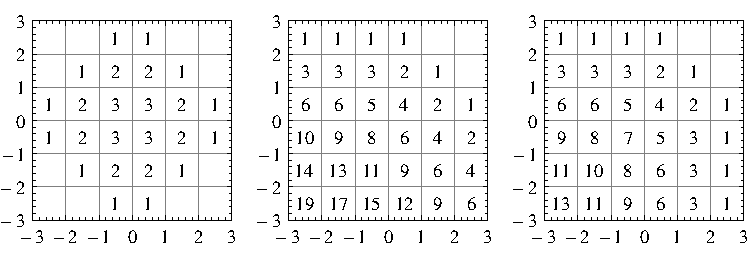
\includegraphics[width=130mm]{figures/irrep-verma-pverma}$
\end{lstlisting}

As we already stated properties of a module are encoded by its singular element. Function \lstinline{singularElement[m_module]} returns singular element of a module as \lstinline{formalElement} datastructure. Character (up to \lstinline{limit} for (parabolic) Verma modules) is returned by the function \lstinline{character[m_module]}. Direct sum of modules is a module and we use natural notation
\begin{lstlisting}[mathescape=true]
im1=makeIrreducibleModule[$B_{2}$][weight[$B_{2}$][2,1]];
im2=makeIrreducibleModule[$B_{2}$][weight[$B_{2}$][1,2]];
textPlot[im1$\oplus$ im2]
$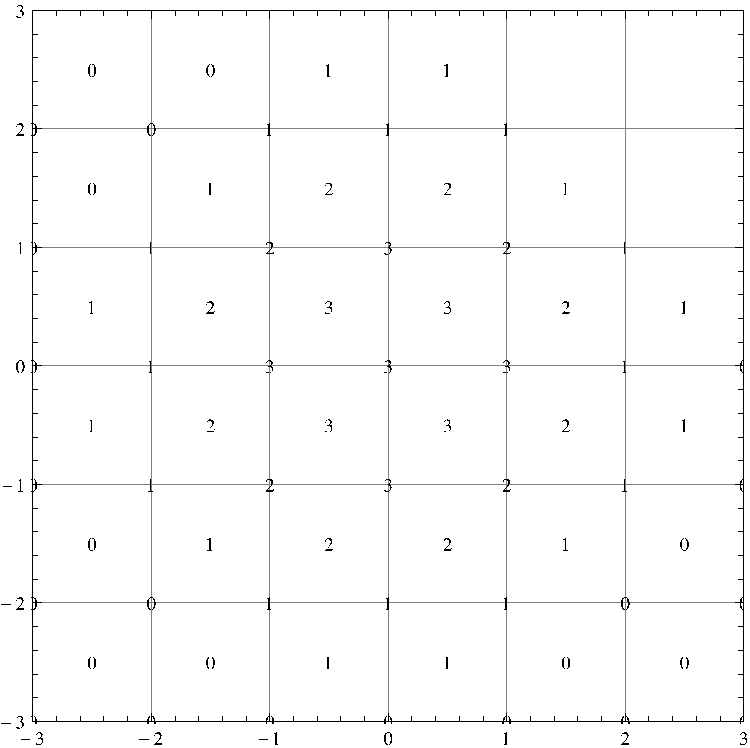
\includegraphics[width=60mm]{figures/irrep-sum}$
\end{lstlisting}

The tensor product is also implemented but only for finite-dimensional Lie algebras, since tensor product of affine Lie algebra modules leads to rich new structures \cite{kazhdan1994tensor3,kazhdan1993tensor1,kazhdan1993tensor2} which are out of the scope of the present paper.
\begin{lstlisting}[mathescape=true]
textPlot[makeIrreducibleModule[$A_{1}$][5]$\otimes$ makeIrreducibleModule[$A_{1}$][3]];
$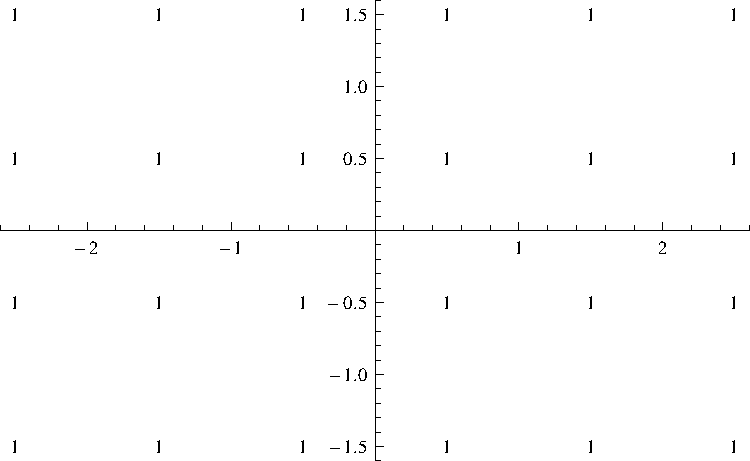
\includegraphics[width=60mm]{figures/tensor-product}$
\end{lstlisting}
\section{Computational algorithms}
\label{sec:comp-algor}
   
As we have already stated in section \ref{sec:high-weight-modul} there exist two recurrent relations which can be used to calculate weight multiplicities in irreducible modules. Both algorithms proceed in the following way to calculate weight multiplicities:
\begin{enumerate}
\item Create the list of weights in the main Weyl chamber by subtracting all possible combinations of simple roots from the highest weight (e.g. for finite-dimensional algebra subtract $\alpha_{1}$ from $\mu$ while inside $\bar C$, then subtract $\alpha_{2}$ from all the weights already obtained etc).
\item Sort the list of weights by their product with the Weyl vector.
\item Use a recurrent formula. If the weight required for recurrent computation is outside the main chamber use the Weyl symmetry.
\end{enumerate}
The difference in the performance of algorithms is in the number of previous values required to get the multiplicity of weight under consideration. For  the Weyl formula based recurrent relation \eqref{eq:14} it is constant and equal to the number of elements in the Weyl group (if we are far from the boundary of representation diagram). When the Freudenthal formula \eqref{eq:15} is used number of previous values grows with the distance from the external border of representation. So the Freudenthal formula is faster if the weight is close to the border or the rank of the algebra and the size of Weyl group is large \cite{moody1982fast}.
Note that the Freudenthal formula is valid for irreducible modules only, so it can not be used to study (generalized) Verma modules.

We have made some experiments with our implementations of the Freudenthal formula and formula \eqref{eq:15} and have got Figure  \ref{fig:freudenthal-racah-times}, which depicts the dependence of the computation time on the number of weights in a module.

\begin{figure}[h]
  \noindent\centering{
    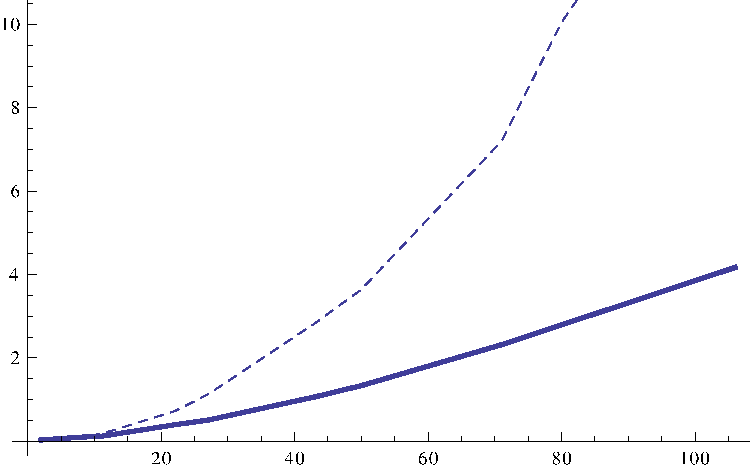
\includegraphics[width=80mm]{figures/timing}
  }
  \caption{Running time of algorithms based on the Freudenthal formula \eqref{eq:15} (dashed) and recurrent relation \eqref{eq:14} (solid) with the number of weights in $\bar C$ for calculation of multiplicities in representations of $B_{2}$.}
\label{fig:freudenthal-racah-times}

\end{figure}

In the calculation of branching coefficients the application of the Freudenthal formula requires a complete construction of formal characters of an algebra module and all the representations of a subalgebra. It is impractical when the rank of algebra and subalgebra are big, for example for maximal subalgebras.

Alternative algorithm which was presented in the paper \cite{2010arXiv1007.0318L}  contains the following steps:

\begin{enumerate}
\item  Construct the root system $\Delta _{\af}$ for the embedding $%
\af\rightarrow \frak{g}$.

\item  Select all the positive roots $\alpha \in \Delta ^{+}$ orthogonal
to  $\af$, i.e. form the set $\Delta_{\afb }^{+}$.

\item  Construct the set $\Gamma _{\af\rightarrow \frak{g}}$. Relation
 (\ref{eq:6}) defines the sign function
 $s(\gamma)$ and the set $\Phi_{\af\subset \frak{g}}$ where the lowest weight
 $\gamma_0$ is to be subtracted to get the fan:
 $\Gamma _{\af\rightarrow \frak{g}}=\left\{ \xi -\gamma _{0}|\xi \in \Phi _{%
\af\subset \frak{g}}\right\} \setminus \left\{ 0\right\}$.

\item  Construct the set $\widehat{\Psi ^{(\mu )}}=\left\{ w (\mu +\rho
)-\rho ;\;w \in W\right\} $ of singular weights for the $\frak{g}$%
-module $L^{(\mu )}$.

\item  Select the weights $\left\{ \mu _{\widetilde{\af_{\perp }}%
}\left( w\right) =\pi _{\widetilde{\af_{\perp }}}\left[ w(\mu +\rho
)-\rho \right] -\mathcal{D}_{\af_{\perp }}\in \overline{C_{\widetilde{%
\af_{\perp }}}}\right\} $. Since the set $\Delta_{\afb }^{+}$ is fixed
we can easily check wether the weight $\mu _{\widetilde{\af_{\perp }}%
}\left( w\right) $ belongs to the main Weyl chamber $\overline{C_{\widetilde{%
\af_{\perp }}}}$ (by computing its scalar product with the fundamental
weights of $\afb^{+}$).

\item  For the weights $\mu _{\widetilde{\af_{\perp }}}\left( w\right) $
calculate dimensions of the corresponding modules, $\mathrm{\dim }\left(
L_{\widetilde{\af_{\perp }}}^{\mu _{\widetilde{\af_{\perp }}%
}\left( u\right) }\right) $, using the Weyl dimension formula and construct
the singular element $\Psi ^{\left( \mu \right) }_{\left(  \af, \afb \right)}$.

\item  Calculate the anomalous branching coefficients using 
recurrent relation (\ref{recurrent-rel}) and select among them those
corresponding to the weights in the main Weyl
chamber $\overline{C_{\af}}$.
\end{enumerate}

We can speed up the algorithm by
one-time computation of the representatives of the conjugate classes $%
W/W_{\afb }$.


Consider the regular embedding $B_{2}\subset B_{4}$. In this case the fan consists of 24 elements. In order to decompose $B_{4}$ module we need to construct the subset of singular weights of the module which projects to the main Weyl chamber of the subalgebra $B_{2}$. The full set of singular weights consists of 384 elements. The required subset contains at most 48 elements. So the time for the construction of this required subset is negligible if the number of branching coefficients is greater than that. We may estimate the total number of required operations for the computation of branching coefficients as the product of the number of elements in the main Weyl chamber of a subalgebra with non-zero branching coefficients and the number of elements in the fan. In the case of a direct algorithm we need to compute the multiplicities for each module in the decomposition, so the number of operations grows faster than the square of the number of elements in the main Weyl chamber of a subalgebra with non-zero branching coefficients. 

To further illustrate this performance issue we include Figure \ref{fig:branching} where we show the time required for computations of branching coefficients for $B_{3}\subset B_{4}$.

\begin{figure}[h]
  \noindent\centering{
   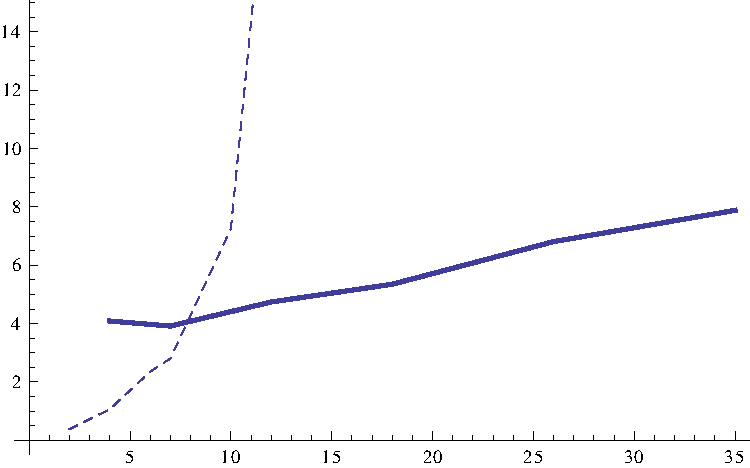
\includegraphics[width=100mm]{figures/branching-timing}
  }
  \caption{Running time of algorithms based on the Freudenthal formula \eqref{eq:15} (dashed) and recurrent relation \eqref{recurrent-rel} (solid) with the number of weights in $\bar C$ for calculation of branching coefficients for $B_{3}\subset B_{4}$.}
  \label{fig:branching}
\end{figure}

\section{Examples}
\label{sec:examples}
In this section we present some examples of computations available with {\bf Affine.m} with the code required to produce these results.

\subsection{Tensor product decompositon for finite-dimensional Lie algebras}
\label{sec:tens-prod-decomp}

Computation of fusion coefficients for the decomposition of tensor product of highest-weight modules to the direct sum of irreducible modules has numerous applications in physics. For example, we can consider the spin of a composite system such as an atom. Another interesting example is integrable spin chain consisting of $N$ particles with the spins living in some representation $L$ of a Lie algebra $\gf$ with a $\gf$-invariant Hamiltonian $H$, describing the nearest-neighbour spin-spin interaction. In order to solve such a system, i.e. to find eigenstates of the Hamiltonian, we need to decompose $L^{\otimes N}$ into the direct sum of irreducible $\gf$-modules of lower dimension and diagonalize the Hamiltonian on these modules.

For fundamental representations of simple Lie algebras it is sometimes possible to get an analytic result describing the dependence of decomposition coefficients on $N$ (See \cite{LyakhovskyPostnova2011}). Our code provides numerical values and can be used to check this analytic results.

Consider a tensor power of $B_{2}$ the first fundamental representation $\left(L^{[1,0]}\right)^{\otimes 4}$. Decomposition coefficients are just the branching
 coefficients for the tensor power module reduced to the diagonal subalgebra $B_{2}\subset B_{2}\oplus B_{2}\oplus B_{2}\oplus B_{2}$. So the following code calculates these coefficients:
\begin{lstlisting}[mathescape=true]
fm = makeIrreducibleModule[$B_{2}$][1, 0];
tp = ((fm$\otimes$ ]fm)$\otimes$ fm)$\otimes$]fm;
subs = makeFiniteRootSystem[
  {1/4*{1, -1, 1, -1, 1, -1, 1, -1}, 
   1/4*{0, 1, 0, 1, 0, 1, 0, 1}}];
bc = branching[tp, subs];
{bc[#], dynkinLabels[subs][#]} & /@ bc[weights]
\end{lstlisting}
It produces a list of highest weights and tensor product decomposition coefficients:
\begin{lstlisting}
{{1, {4, 0}}, {3, {2, 2}}, {0, {3, 0}}, 
{2, {0, 4}}, {3, {1, 2}}, {6, {2, 0}}, 
{6, {0, 2}}, {1, {1, 0}}, {3, {0, 0}}}]
\end{lstlisting}

Returning to the problem of spin chain Hamiltonian diagonalization we can see that instead of diagonalizing operator in space of dimension $625$ we can diagonalize operators in the spaces of dimensions $55, 81, 30, 35, 35, 14, 10, 5, 1$.

\subsection{Branching and parabolic Verma modules}
\label{sec:branch-parab-verma}

We illustrate the generalized BGG-resolution by the diagrams of $G_{2}$ parabolic Verma modules which appear in the decomposition of irreducible module $L^{[1,1]}_{G_{2}}$:
\begin{equation}
\mathrm{ch}\left( L^{\mu }\right) =\sum_{u\in U}\;e^{\mu _{\aft}\left(
u\right) }\epsilon (u)\mathrm{ch}M_{I}^{\mu _{\frak{a}_{\perp }}\left(
u\right) }.  \label{char-in-gen-verma-mod}
\end{equation}
The character of $L^{[1,1]}$ is presented in Figure \ref{branching-bgg}, characters of the generalized Verma modules in decomposition \eqref{char-in-gen-verma-mod} are shown in Figure \ref{g2-pverma}. Characters in the upper row appear in \eqref{char-in-gen-verma-mod} with positive sign and in the lower row -- with negative.


\begin{figure}[h]
  \noindent\centering{
    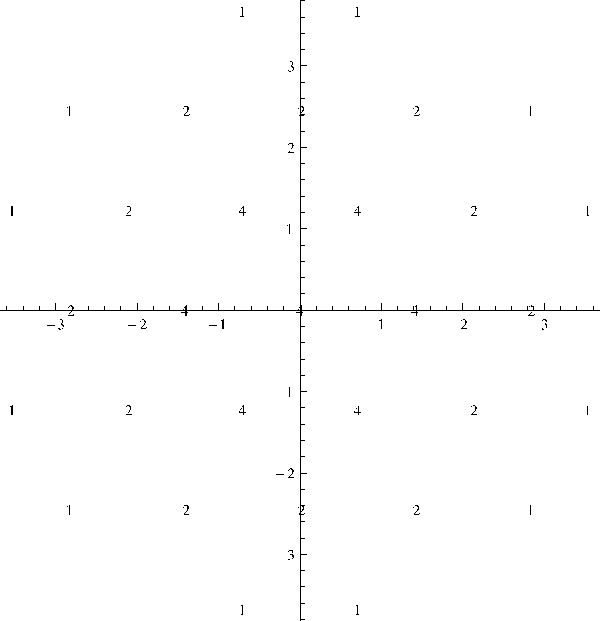
\includegraphics[width=80mm]{figures/G2-irrep}
  }
  \caption{Character of the irreducible $G_{2}$-module $L^{[1,1]}$}
  \label{branching-bgg}
\end{figure}
\begin{figure}[h]
  \noindent\centering{
    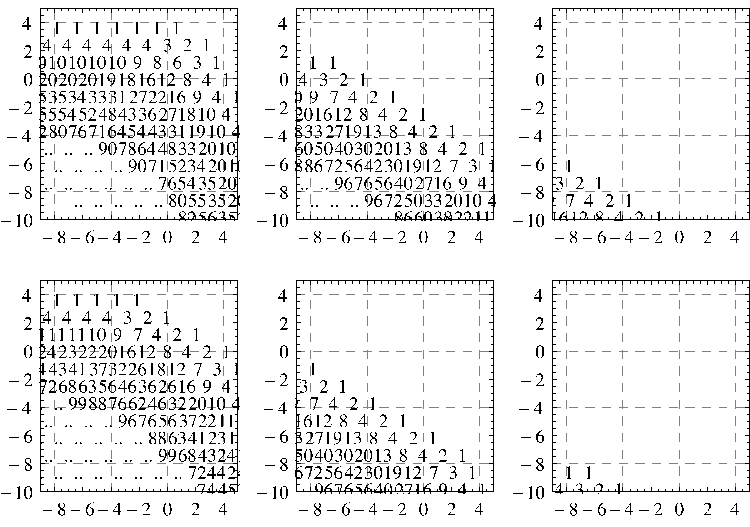
\includegraphics[width=150mm]{figures/G2-pverma}
  }
  \caption{Characters of $G_{2}$ generalized Verma modules appearing in the decomposition of $L^{[1,1]}$. Parabolic Verma modules in the upper row appear in the decomposition with a positive sign, in the lower row -- with a negative.}
  \label{g2-pverma}
\end{figure}

\subsection{String functions of affine Lie algebras and CFT models}
\label{sec:string-funct-affine}

String functions can be used to present formal characters of affine Lie algebra highest weight representation. They have interesting analytic and modular properties \cite{kac1990idl,kac1988modular,kac1984infinite}.

{\bf Affine.m} produces power series decomposition for string functions. Consider an affine Lie algebra $\hat{sl(3)}=\hat A_{2}$ and its highest weight module $L^{(1,0,0)}$. To get the string functions we can use the code:
\begin{lstlisting}[mathescape=true]
stringFunctions[$\hat A_2$,{1,1,2}]
{{0, 0, 4}, 
  $2 q + 10 q^2 + 40 q^3 + 133 q^4 + 398 q^5 + 1084 q^6 + 2760 q^7 + 6632 q^8 + 15214 q^9 + 33508 q^{10}$}, 
{{0, 3, 1}, 
  $2 q + 12 q^2 + 49 q^3 + 166 q^4 + 494 q^5 + 1340 q^6 + 3387 q^7 + 8086 q^8 + 18415 q^9 + 40302 q^{10}$}, 
{{1, 1, 2}, 
  $1 + 6 q + 27 q^2 + 96 q^3 + 298 q^4 + 836 q^5 + 2173 q^6 + 5310 q^7 + 12341 q^8 + 27486 q^9 + 59029 q^{10}$}, 
{{2, 2, 0}, 
  $1 + 8 q + 35 q^2 + 124 q^3 + 379 q^4 + 1052 q^5 + 2700 q^6 + 6536 q^7 + 15047 q^8 + 33248 q^9 + 70877 q^{10}$}, 
{{3, 0, 1}, 
  $2 + 12 q + 49 q^2 + 166 q^3 + 494 q^4 + 1340 q^5 + 3387 q^6 + 8086 q^7 + 18415 q^8 + 40302 q^9 + 85226 q^{10}$}
\end{lstlisting}
Similarly for the affine Lie algebra $\hat G_{2}$ we get
\begin{lstlisting}[mathescape=true]
stringFunctions[$\hat G_2$,{1,1,0}]
{{2, 0, 0}, 
  $1 + 8 q + 37 q^2 + 138 q^3 + 431 q^4 + 1227 q^5 + 3208 q^6 + 7901 q^7$}, 
{{0, 0, 1}, 
  $3 q + 18 q^2 + 73 q^3 + 247 q^4 + 736 q^5 + 2000 q^6 + 5070 q^7$}, 
{{1, 1, 0},
  $1 + 7 q + 32 q^2 + 117 q^3 + 370 q^4 + 1055 q^5 + 2780 q^6 + 6880 q^7$}, 
{{0, 2, 0}, 
  $3 q + 15 q^2 + 63 q^3 + 210 q^4 + 633 q^5 + 1725 q^6 + 4407 q^7$}
\end{lstlisting}

\subsection{Branching functions and coset models of conformal field theory}
\label{sec:branch-funct-coset}

It is believed that most rational models of CFT can be obtained from cosets $G/A$ corresponding to the embedding $\af\subset\gf$. These models can be studied as gauge theories \cite{Hwang:1994yr, hwang1993brst}.

Branching functions for an embedding $\af\subset\gf$ are the partition functions of CFT on the torus (see \cite{difrancesco1997cft}).

As a first example we show how to construct branching functions for the embedding $\hat A_{1}\to \hat B_{2}$ up to the tenth grade:
\begin{lstlisting}[mathescape=true]
branchingFunctions[$\hat B_{2}$,makeAffineExtension[makeFiniteRootSystem[{{1, 1}}]], {1, 1, 1}]

 {{3, 0}, 
  $2 + 14 q + 52 q^2 + 154 q^3 + 410 q^4 + 994 q^5 + 2248 q^6 + 4832 q^7 + 9934 q^8 + 19680 q^9 + 37802 q^{10}$},
 {{2, 1}, 
  $4 + 20 q + 72 q^2 + 220 q^3 + 584 q^4 + 1424 q^5 + 3248 q^6 + 7012 q^7 + 14488 q^8 + 28844 q^9 + 55616 q^{10}$},
 {{0, 3}, 
  $4 q + 20 q^2 + 68 q^3 + 200 q^4 + 516 q^5 + 1224 q^6 + 2736 q^7 + 5808 q^8 + 11820 q^9 + 23236 q^{10}$},
 {{1, 2}, 
  $2 + 14 q + 54 q^2 + 168 q^3 + 462 q^4 + 1148 q^5 + 2656 q^6 + 5812 q^7 + 12130 q^8 + 24358 q^9 + 47328 q^{10}$}
\end{lstlisting}

Another example demonstrates the computation of branching functions for the regular embedding $\hat B_{2}\subset \hat C_{3}$:
\begin{lstlisting}[mathescape=true]
sub=makeAffineExtension[parabolicSubalgebra[$C_{3}$][2,3]];
branchingFunctions[$\hat C_{3}$,sub, {2, 0, 0, 0}]

{{0, 1, 0}, 
  $2 q - 20 q^3 + 24 q^4 + 82 q^5 - 320 q^6 + 108 q^7$}, 
{{1, 0, 0}, 
  $1 - q - 8 q^2 + 19 q^3 + 16 q^4 - 156 q^5 + 205 q^6 + 640 q^7$}, 
{{0, 0, 1}, 
  $q - 5 q^3 + 7 q^5$}
\end{lstlisting}

\section{Conclusion}
\label{sec:conclusion}
We have presented the package {\bf Affine.m} for computations in representation theory of finite-dimensional and affine Lie algebras. It can be used to study Weyl symmetry, root systems, irreducible, Verma and parabolic Verma modules of finite-dimensional and affine Lie algebras.  In the present paper we have also discussed main ideas used for an implementation of the package and described most important notions of representation theory required to use {\bf Affine.m}. 

We have demonstrated that recurrent approach based on the Weyl character formula is not only useful for calculations but also allows to establish connections with the (generalized) Bernstein-Bernstein-Gelfand resolution. 

Also we have presented examples of computations with this package connected with problems of physics and mathematics. 

In future versions of our software we are going to treat twisted affine Lie algebras, extended affine Lie algebras and provide more direct support for tensor product decompositions. 

\section*{Acknowledgements}
\label{sec:acknowledgements}
I thank V.D. Lyakhovsky and O.Postnova for discussions and helpful comments.

The work is supported by the Chebyshev Laboratory
(Department of Mathematics and Mechanics, Saint-Petersburg State
University) under the grant 11.G34.31.0026 of the Government of the
Russian Federation.


%% The Appendices part is started with the command \appendix;
%% appendix sections are then done as normal sections
%\appendix

\section{Software package}
\label{package}
The package can be freely downloaded from \url{http://github.com/naa/Affine}. To get the development code use the command
\begin{lstlisting}[language=bash]
 git clone git://github.com/naa/Affine.git
\end{lstlisting}

Contents of the package:
\begin{verbatim}
    Affine/                                root folder
      demo/                                  demonstrations
        demo.nb                                demo notebook
        paper.nb                               code for the paper
      doc/                                 documentation folder
        figures/                             figures in paper 
          timing.pdf                           diagram showing performance
          branching-timing.pdf                 ...  for branching coefficients  
          irrep-sum.pdf                        sum of B2 irreps
          irrep-verma-pverma.pdf               irrep, Verma, (p)Verma for B2
          G2-irrep.pdf                         irrep for G2
          G2-pverma.pdf                        parabolic Verma for G2
          tensor-product.pdf                   tensor product of A1-modules
        bibliography.bib                     bibliographic database
        paper.pdf                            present paper
        paper.tex                            paper source
        TODO.org                             list of issues
      src/                                 source folder
        affine.m                             main software package
      tests/                               unit tests folder
        tests.m                              unit tests
      README.markdown                      installation and usage notes
\end{verbatim}


%% References
%%
%% Following citation commands can be used in the body text:
%% Usage of \cite is as follows:
%%   \cite{key}         ==>>  [#]
%%   \cite[chap. 2]{key} ==>> [#, chap. 2]
%%

%% References with bibTeX database:

  %   \section*{References}
  %   \label{sec:references}
  %   
  %   
  %   \bibliography{bibliography}
  %   \bibliographystyle{phcpc}
  %   %\bibliographystyle{model1-num-names}
  %   
  %   
  %   %% Authors are advised to submit their bibtex database files. They are
  %   %% requested to list a bibtex style file in the manuscript if they do
  %   %% not want to use elsarticle-num.bst.
  %   
  %   %% References without bibTeX database:
  %   
  %   % \begin{thebibliography}{00}
  %   
  %   %% \bibitem must have the following form:
  %   %%   \bibitem{key}...
  %   %%
  %   
  %   % \bibitem{}
  %   
  %   % \end{thebibliography}
  %   
  %   
  %   

%%
%% End of file
%%% Local Variables: 
%%% mode: latex
%%% TeX-master: "thesis"
%%% End: 
